\documentclass[a4paper, 11pt]{article}
\usepackage{comment} % enables the use of multi-line comments (\ifx \fi) 
\usepackage{lipsum} %This package just generates Lorem Ipsum filler text. 
\usepackage{fullpage} % changes the margin
\usepackage{epsfig}

\begin{document}
%Header-Make sure you update this information!!!!
\noindent
\large\textbf{Project Report} \hfill \textbf{Abhishek Srivastava} \\
\normalsize CS229 Machine Learning\hfill Student Id: 861307778 \\
Prof. Christian Shelton \hfill Date: 12/08/2016 \\

\hrule

\section*{Problem Statement}
Given a handwritten alphabet dataset our goal is to produce a model based on the training data, which predicts the target values of the test data given only the test data attributes.

\section*{Initial Approach}
I choose Support Vector Machines(SVM) as my classifier for the following reasons:
\begin{itemize}
	\item It is very effective in high dimensional spaces.
	\item It uses a subset of training points in the decision  function, so it is also memory efficient.
	\item Different Kernel functions can be specified for the decision function.
\end{itemize}
After selecting the SVM as my classifier I used following procedure:
\begin{itemize}
	\item Read the data and split it 80\% training data and 20\% test data with random sampling to make dataset more chaotic.
	\item I tried 5 Kernels : `Linear', `RBF' , `Polynomial degree = 2', `Polynomial degree = 3' and `Sigmoid'. Table 1 shows the accuracy of each kernel.
	\item Then I tested the classifier with the held out testing data and choose `RBF' kernel to work further with because it gave the highest accuracy.
\end{itemize}

One thing also I observed that both polynomial kernel performed very poorly with respect to other kernels the reason may be of happening this is their kernel values may be very large because the degree is large. The accuracy of linear kernel was close with RBF kernel, the reason for that can be as dimension increases they start to behave more or less same. So we could have used linear kernel as well. But the reason for choosing `RBF' kernel is that this kernel can map the samples into higher dimensional space so it can handle the cases where relation between class labels and the attributes are nonlinear and I was also planning to do dimension reduction.\cite{svmguide}
\section*{Analysis of Initial Approach}

With randomly sampling the data I was getting 0.8400 accuracy with training data and with 0.8290 accuracy with testing data. The reasons of getting this low accuracy can be following:
\begin{itemize}
	\item Given data is very high dimensional(d = 129) so there is a possibility that many of the features can be unnecessary. So feature reduction can improve the accuracy of the classifier.
	\item Unbalance classes can be one the reasons. If sampling is unbalanced then classifier can be biased toward particular classes. To check this I plotted the confusion matrix and found out that some alphabet classes were little unbalanced. Classes: `a', `e', `i', `l', `n', `o' and `u' were in more number with respect to the other classes. So one more thing I can try was to balance the class while fitting the classifier. 
	\item While fitting SVM the classifier takes default value of `C' as 1. `C' parameter tells the SVM optimization how much you want to avoid misclassifying each training example. `C' parameter trades off misclassification of training examples against simplicity of the decision surface. So choosing better `C' can improve the classifier.
	\item Other parameter which can be adjusted to improve the classifier is `gamma'. The `gamma' parameter defines how far the influence of a single training example. By default value of `gamma' is 1/number of samples. 
\end{itemize} 
I also plotted Learning curve of the whole data using 'RBF' kernel to just check that if it is getting overfitted or not. Figure 1 shows the plotted graph of accuracy vs size of the training data with default C and gamma.
.\\

\begin{table}
	\centering
	\caption{Performance of all kernels in fraction of correct classification on test data.}
	\begin{tabular}{|c|l|} \hline
		Kernel Name&Accuracy\\ \hline
		Linear & 0.8242 \\ \hline
		RBF & 0.8290 \\ \hline
		Polynomial degree = 2 & 0.7160 \\ \hline
		Polynomial degree = 3 & 0.4804\\ \hline
		Sigmoid & 0.7986\\ \hline
	\end{tabular}
\end{table}
\begin{figure}
	\centering
	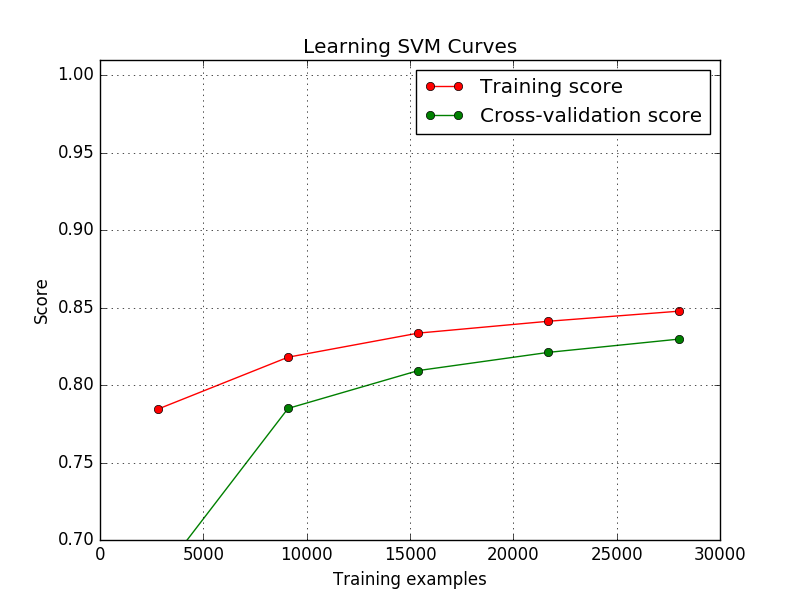
\epsfig{file=learning_curve.png, height=2.5in, width=3.5in}
	\caption{Learning Curve of Accuracy vs Number of Training examples.}
\end{figure}
\section*{Improvement on Intial Analysis}
\begin{itemize}
	\item Reducing the dimension: I used the PCA to reduce the dimensionality of the training data. I tested different fraction which gave different accuracies. I selected n\_components values as 0.7 as it gave the highest accuracy. Table 2 shows the accuracy with different n\_component values.
	\item Balancing Unbalanced Classes: I passes class\_weight as `balanced' which balance the classes to train the classifier. But it resulted decreasing the accuracy (0.8212)rather than improvement. I tested it again after applying PCA as well but it again decreased the improvement. So I dropped this method.
	\item `C' and `gamma' values: I used grid search method to find the appropriate value of C and gamma on the whole data. It runs each permutation with cross-validation to return the best C \& gamma value pair. After running this method I got C = `10' and gamma as `0.01778' as appropriate values for this dataset with a score of 0.88. But to get more precise result I again used search grid with gamma range between 0.01 to 1 , I got 0.1 as the best result.
\end{itemize}
\begin{table}
	\centering
	\caption{Performance of different PCA with different n\_components value.}
	\begin{tabular}{|c|c|c|c|c|c|l|} \hline
		n\_component&1&0.9&0.8&0.7&0.6&0.5\\ \hline
		Accuracy&0.8290&0.8527&0.8576&0.8624&0.8596&0.8507\\ \hline
	\end{tabular}
\end{table}
\section*{Final Approach}
In the final approach Training and Testing data is reduced to n\_components = 0.7 using PCA function to reduce the high dimensionality of the data. \\
Then I trained a SVM Classifier with following parameters:
\begin{itemize}
	\item Kernel = `RBF'
	\item C = `10'
	\item gamma = `0.1'.
\end{itemize}
\section*{Final Analysis}
After finding all the parameters I tested the same classifier over whole dataset and used cross validation score to calculate the accuracy I got the 0.8996 accuracy.

Future steps which can be taken are :
\begin{itemize}
	\item Neural Network can be used which is much more capable of handling complex data like this.
	\item Better kernel can be tested or may be custom kernel can be designed to tackle this specific problem.
	\item Grid search takes too much time, so much better algorithm can be designed to calculate C and gamma in better time. 
\end{itemize} 
\begin{thebibliography}{9} 
\bibitem{svmguide}Chih-Wei Hsu, Chih-Chung Chang, and Chih-Jen Lin. 2003. \emph{A Practical Guide to Support Vector Classification.}  Department of Computer Science, National Taiwan University. 
\bibitem{Scikit} Scikit-learn: Used packages as model\_selection, svm, decomposition, metrics \& externals. \emph{http://scikit-learn.org/}
\bibitem{Numpy} Numpy: Used numpy package to manipulate arrays such as mean, std, storing array in file etc . \emph{http://docs.scipy.org/}
\end{thebibliography}

\end{document}
